\let\negmpace\undefined
\let\negthickspace\undefined
\documentclass[journal]{IEEEtran}
\usepackage[a5paper, margin=10mm, onecolumn]{geometry}
%\usepackage{lmodern} % Ensure lmodern is loaded for pdflatex
\usepackage{tfrupee} % Include tfrupee package
\setlength{\headheight}{1cm} % Set the height of the header box
\setlength{\headsep}{0mm}     % Set the distance between the header box and the top of the text
\usepackage{gvv-book}
\usepackage{gvv}
\usepackage{cite}
\usepackage{amsmath,amssymb,amsfonts,amsthm}
\usepackage{algorithmic}
\usepackage{graphicx}
\usepackage{textcomp}
\usepackage{xcolor}
\usepackage{txfonts}
\usepackage{listings}
\usepackage{enumitem}
\usepackage{mathtools}
\usepackage{gensymb}
\usepackage{comment}
\usepackage[breaklinks=true]{hyperref}
\usepackage{tkz-euclide} 
\usepackage{listings}
% \usepackage{gvv}                                        
\def\inputGnumericTable{}                                 
\usepackage[latin1]{inputenc}                                
\usepackage{color}                                            
\usepackage{array}                                            
\usepackage{longtable}                                       
\usepackage{calc}                                             
\usepackage{multirow}                                         
\usepackage{hhline}                                           
\usepackage{ifthen}                                           
\usepackage{lscape}
\renewcommand{\thefigure}{\theenumi}
\renewcommand{\thetable}{\theenumi}
\setlength{\intextsep}{10pt} % Space between text and floats
\numberwithin{equation}{enumi}
\numberwithin{figure}{enumi}
\renewcommand{\thetable}{\theenumi}
\title{Assignment4}
\author{Teja Vardhan Shannu}
\date{August 2024}

\begin{document}
\maketitle

\section*{Question}
Given the vertices of a triangle \( PQR \) as \( P(2, 2) \), \( Q(-4, -4) \), and \( R(5, -8) \), find the length of the median through \( R \).

\section*{Solution}

We are given the vertices of triangle \( PQR \) as follows:
\begin{align}
P(2, 2), \quad Q(-4, -4), \quad R(5, -8)
\end{align}
We are asked to find the length of the median through vertex \( R \), using the matrix approach.

\section*{Step 1: Find the Midpoint of \( PQ \)}
The midpoint \( M \) of the line segment \( PQ \) is calculated as:
\begin{align}
M = \left( \frac{P_x + Q_x}{2}, \frac{P_y + Q_y}{2} \right)
\end{align}
Substituting the coordinates of \( P(2, 2) \) and \( Q(-4, -4) \):
\begin{align}
M = \left( \frac{2 + (-4)}{2}, \frac{2 + (-4)}{2} \right) = (-1, -1)
\end{align}

\section*{Step 2: Represent Points as Column Vectors}

We now represent the points \( R \) and \( M \) as column vectors:
\begin{align}
\mathbf{R} = \begin{pmatrix} 5 \\ -8 \end{pmatrix}, \quad \mathbf{M} = \begin{pmatrix} -1 \\ -1 \end{pmatrix}
\end{align}

\section*{Step 3: Find the Vector from \( R \) to \( M \)}

To find the vector from \( R \) to \( M \), we subtract the vector \( \mathbf{M} \) from \( \mathbf{R} \):
\begin{align}
\mathbf{RM} = \mathbf{R} - \mathbf{M} = \begin{pmatrix} 5 \\ -8 \end{pmatrix} - \begin{pmatrix} -1 \\ -1 \end{pmatrix} = \begin{pmatrix} 5 - (-1) \\ -8 - (-1) \end{pmatrix} = \begin{pmatrix} 6 \\ -7 \end{pmatrix}
\end{align}

\section*{Step 4: Find the Length of the Median}

The length of the median through \( R \) is the magnitude of the vector \( \mathbf{RM} \), which is calculated as:
\begin{align}
|\mathbf{RM}| = \sqrt{6^2 + (-7)^2} = \sqrt{36 + 49} = \sqrt{85}
\end{align}

Thus, the length of the median through \( R \) is \( \sqrt{85} \) units.


\begin{figure}[h!]
  \hspace{-1cm}
  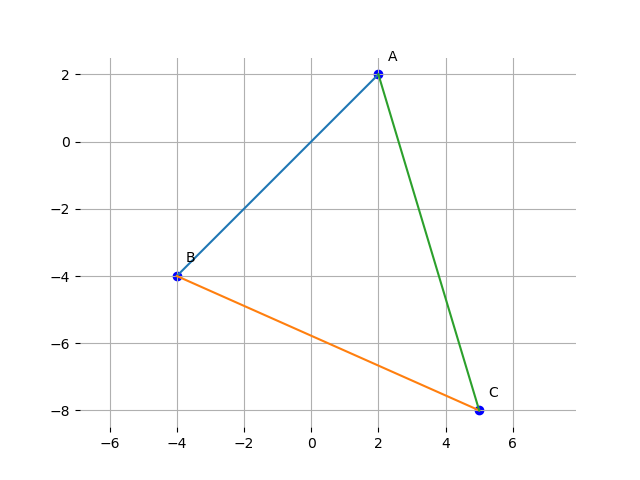
\includegraphics[width=1.2\textwidth]{Figure_2.png}
  
  \caption{The plot of the points }
  \label{fig:your_label}
\end{figure}




\end{document}
